Peg Solitaire er et spil hvor en person skal forsøge at fjerne pinde i
et bræt med huller ved at foretage en række træk indtil der kun er en
pind tilbage på brættet. I hvert træk kan en pind fjernes ved at en
nabopind flyttes over pinden til et ledigt hul. For hvert træk
efterlades brættet med en pind færre.

\begin{minipage}{.75\textwidth}
I den klassiske engelske version af spillet Peg Solitaire består
brættet af 33 huller, som til at starte med er fyldt med 32 pinde; det
midterste hul i brættet er ikke udfyldt og opgaven består i at det
netop er det midterste hul, der til slut skal indeholde en pind.
\end{minipage}
\begin{minipage}{.2\textwidth}
  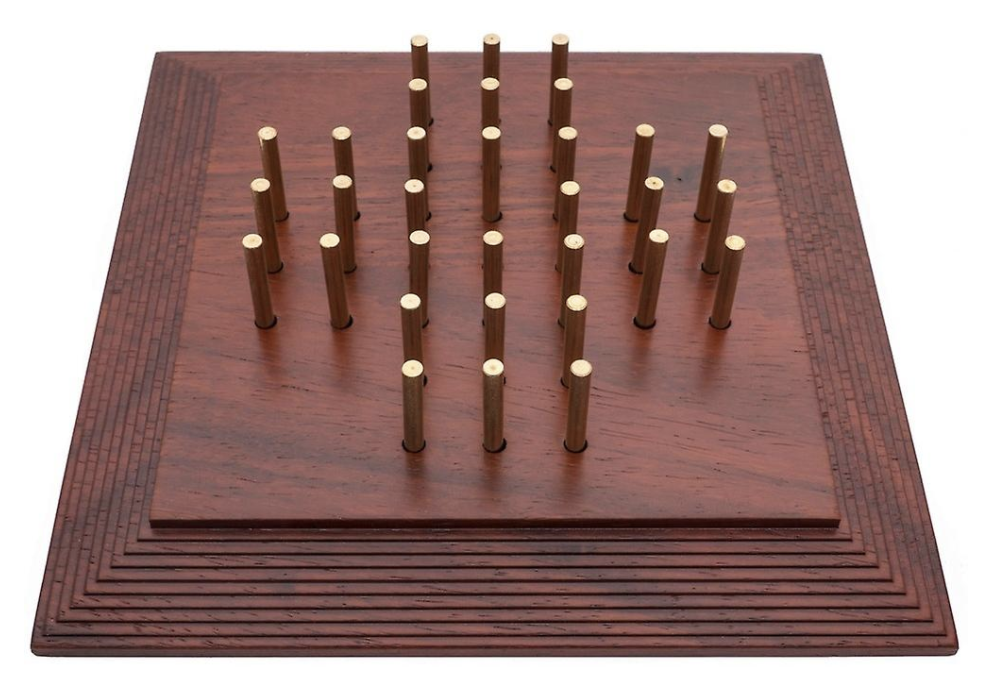
\includegraphics[width=3cm]{solitaire.png}
\end{minipage}
